\chapter*{Приложение 1. Результаты обработки изображения <<Лена>>}
\addcontentsline{toc}{chapter}{Приложение 1. Результаты обработки изображения <<Лена>>}
\begin{figure}[h!]
	\centering
	\begin{subfigure}[t]{0.32\textwidth}
		\centering
		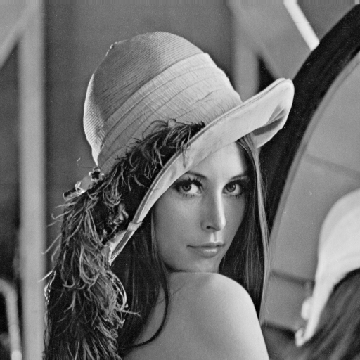
\includegraphics[width=\linewidth]{one-dim-drawn-lena-original}
		\caption{Исходное изображение}
	\end{subfigure}
	\hfill
	\begin{subfigure}[t]{0.32\textwidth}
		\centering
		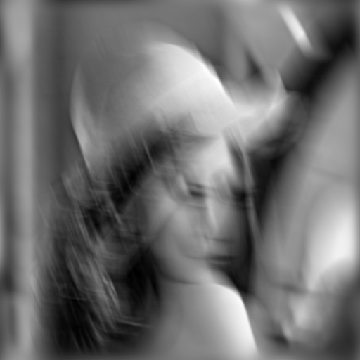
\includegraphics[width=\linewidth]{one-dim-drawn-lena-blurred}
		\caption{смазанное изображение}
	\end{subfigure}
	\hfill
	\begin{subfigure}[t]{0.32\textwidth}
		\centering
		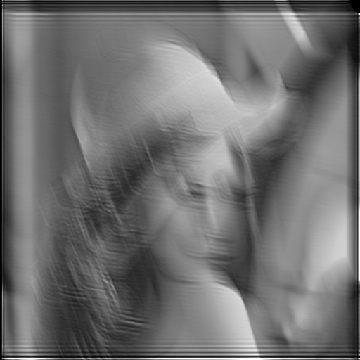
\includegraphics[width=\linewidth]{one-dim-drawn-lena-restored-initial-approx}
		\caption{первое приближение (0; 0), (22.5; 18), (45; 36), PSNR=15.96дБ}
	\end{subfigure}
	\begin{subfigure}[t]{0.32\textwidth}
		\centering
		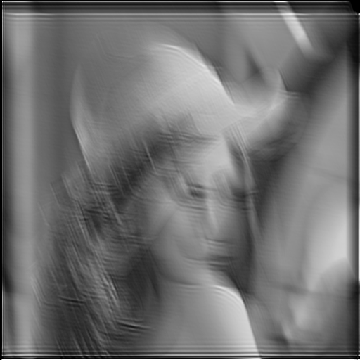
\includegraphics[width=\linewidth]{one-dim-drawn-lena-restored-second-approx}
		\caption{второе приближение (0,0), (4.5; 40.5), (45, 36), PSNR=19.40}
	\end{subfigure}
	\hfill
	\begin{subfigure}[t]{0.32\textwidth}
		\centering
		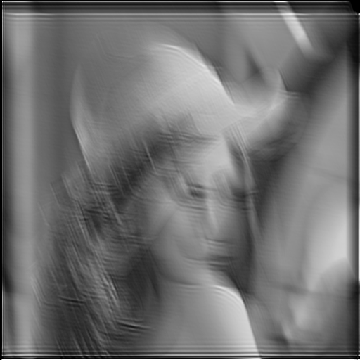
\includegraphics[width=\linewidth]{one-dim-drawn-lena-restored-final}
		\caption{уточнение градиентным спуском (0,0), (4.5; 40.5), (45, 36), PSNR=19.4}
	\end{subfigure}
	\hfill
	\begin{subfigure}[t]{0.32\textwidth}
		\centering
		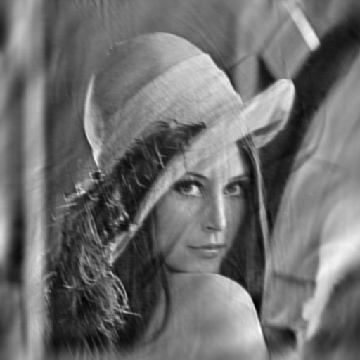
\includegraphics[width=\linewidth]{one-dim-drawn-lena-restored-true-psf}
		\caption{восстановление с <<правильным>> оператором, PSNR=23.36}
	\end{subfigure}
	\label{fig:oneDimDrawnLena}
	\caption{Восстановление изображения искажённого оператором \ref{fig:drawnPsf2}}
\end{figure}

\begin{figure}[h!]
	\centering
	\begin{subfigure}[b]{0.4\textwidth}
		\centering
		
\includegraphics[width=\linewidth]{../input/drawn-psf2}
		\caption{исходный искажающий оператор}
		\label{fig:drawnPsf2}
	\end{subfigure}
	\begin{subfigure}[b]{0.4\textwidth}
		\centering
		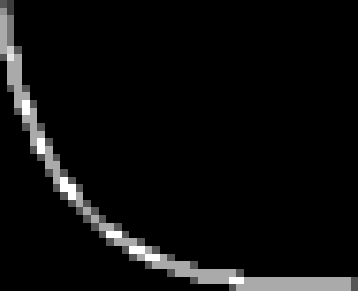
\includegraphics[width=\linewidth]{one-dim-drawn-lena-found-psf}
		\caption{оценка искажающего оператора}
	\end{subfigure}
	\caption{искажающий оператор и его оценка}
\end{figure}
\pagebreak
\chapter*{Приложение 1. Результаты обработки изображения <<Фотограф>>}
\addcontentsline{toc}{chapter}{Приложение 1. Результаты обработки изображения <<Фотограф>>}
\begin{figure}[h!]
	\centering
	\begin{subfigure}[t]{0.32\textwidth}
		\centering
		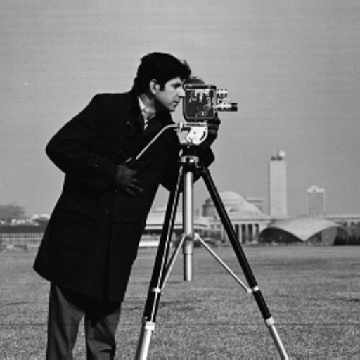
\includegraphics[width=\linewidth]{one-dim-drawn-cameraman-original}
		\caption{Исходное изображение}
	\end{subfigure}
	\hfill
	\begin{subfigure}[t]{0.32\textwidth}
		\centering
		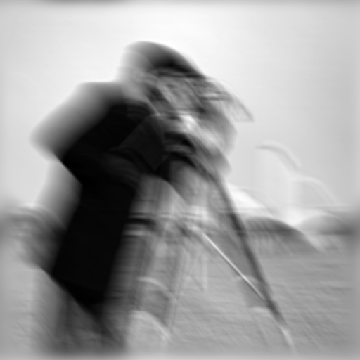
\includegraphics[width=\linewidth]{one-dim-drawn-cameraman-blurred}
		\caption{смазанное изображение}
	\end{subfigure}
	\hfill
	\begin{subfigure}[t]{0.32\textwidth}
		\centering
		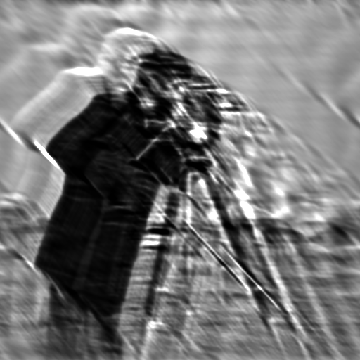
\includegraphics[width=\linewidth]{one-dim-drawn-cameraman-restored-initial-approx}
		\caption{первое приближение (0; 0), (26; 17), (52; 34), PSNR=15.46дБ}
	\end{subfigure}
	\begin{subfigure}[t]{0.32\textwidth}
		\centering
		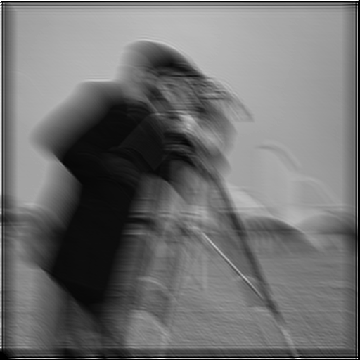
\includegraphics[width=\linewidth]{one-dim-drawn-cameraman-restored-second-approx}
		\caption{второе приближение (0,0), (41.82; -7.21), (52, 34), PSNR=18.22}
	\end{subfigure}
	\hfill
	\begin{subfigure}[t]{0.32\textwidth}
		\centering
		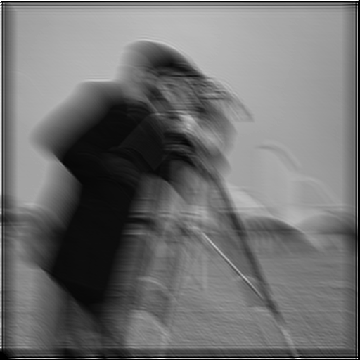
\includegraphics[width=\linewidth]{one-dim-drawn-cameraman-restored-final}
		\caption{уточнение градиентным спуском (0,0), (41.83; -7.61), (51.99, 34.00), PSNR=17.88}
	\end{subfigure}
	\hfill
	\begin{subfigure}[t]{0.32\textwidth}
		\centering
		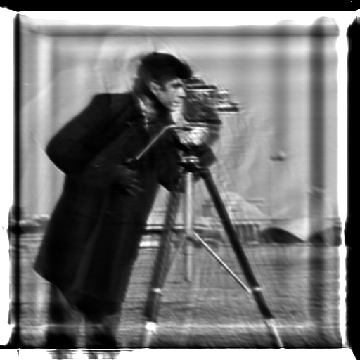
\includegraphics[width=\linewidth]{one-dim-drawn-cameraman-restored-true-psf}
		\caption{восстановление с <<правильным>> оператором, PSNR=21.98}
	\end{subfigure}
	\label{fig:oneDimDrawnCameraman}
	\caption{Восстановление изображения искажённого оператором \ref{fig:drawnPsf3-2}}
\end{figure}

\begin{figure}[h!]
	\centering
	\begin{subfigure}[b]{0.4\textwidth}
		\centering
		
\includegraphics[width=\linewidth]{../input/drawn-psf3}
		\caption{исходный искажающий оператор}
		\label{fig:drawnPsf3-2}
	\end{subfigure}
	\begin{subfigure}[b]{0.4\textwidth}
		\centering
		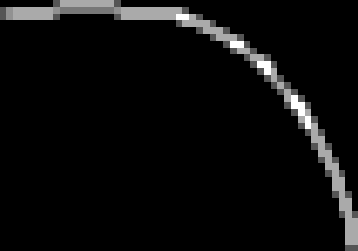
\includegraphics[width=\linewidth]{one-dim-drawn-cameraman-found-psf}
		\caption{оценка искажающего оператора}
	\end{subfigure}
	\caption{искажающий оператор и его оценка}
\end{figure}

\chapter*{Приложение 3. Листинг алгоритмов Люси-Ричардсона и оценки искажения}
\addcontentsline{toc}{chapter}{Приложение 3. Листинг алгоритмов Люси-Ричардсона и оценки искажающего оператора}
\begin{verbatim}
import numpy as np
from scipy.signal import fftconvolve, convolve2d
from numpy.fft import fftn, ifftn
from scipy.stats.stats import pearsonr

def row_correlation(image):
    return pearsonr(image[1:,:].ravel(), image[:-1,:].ravel())[0]
    
def col_correlation(image):
    return pearsonr(image[:,1:].ravel(), image[:,:-1].ravel())[0]


def zero_pad(image, shape, position='corner'):
    """
    Extends image to a certain size with zeros
    Parameters
    ----------
    image: real 2d `numpy.ndarray`
        Input image
    shape: tuple of int
        Desired output shape of the image
    position : str, optional
        The position of the input image in the output one:
            * 'corner'
                top-left corner (default)
            * 'center'
                centered
    Returns
    -------
    padded_img: real `numpy.ndarray`
        The zero-padded image
    """
    shape = np.asarray(shape, dtype=int)
    imshape = np.asarray(image.shape, dtype=int)

    if np.alltrue(imshape == shape):
        return image

    if np.any(shape <= 0):
        raise ValueError("ZERO_PAD: null or negative shape given")

    dshape = shape - imshape
    if np.any(dshape < 0):
        raise ValueError("ZERO_PAD: target size smaller than source one")

    pad_img = np.zeros(shape, dtype=image.dtype)

    idx, idy = np.indices(imshape)

    if position == 'center':
        if np.any(dshape % 2 != 0):
            raise ValueError("ZERO_PAD: source and target shapes "
                             "have different parity.")
        offx, offy = dshape // 2
    else:
        offx, offy = (0, 0)

    pad_img[idx + offx, idy + offy] = image

    return pad_img

def psf2otf(psf, shape):
    """
    Convert point-spread function to optical transfer function.
    Compute the Fast Fourier Transform (FFT) of the point-spread
    function (PSF) array and creates the optical transfer function (OTF)
    array that is not influenced by the PSF off-centering.
    By default, the OTF array is the same size as the PSF array.
    To ensure that the OTF is not altered due to PSF off-centering, PSF2OTF
    post-pads the PSF array (down or to the right) with zeros to match
    dimensions specified in OUTSIZE, then circularly shifts the values of
    the PSF array up (or to the left) until the central pixel reaches (1,1)
    position.
    Parameters
    ----------
    psf : `numpy.ndarray`
        PSF array
    shape : int
        Output shape of the OTF array
    Returns
    -------
    otf : `numpy.ndarray`
        OTF array
    Notes
    -----
    Adapted from MATLAB psf2otf function
    """
    if np.all(psf == 0):
        return np.zeros_like(psf)

    inshape = psf.shape
    # Pad the PSF to outsize
    psf = zero_pad(psf, shape, position='corner')

    # Circularly shift OTF so that the 'center' of the PSF is
    # [0,0] element of the array
    for axis, axis_size in enumerate(inshape):
        psf = np.roll(psf, -int(axis_size / 2), axis=axis)

    # Compute the OTF
    otf = np.fft.fft2(psf)

    # Estimate the rough number of operations involved in the FFT
    # and discard the PSF imaginary part if within roundoff error
    # roundoff error  = machine epsilon = sys.float_info.epsilon
    # or np.finfo().eps
    n_ops = np.sum(psf.size * np.log2(psf.shape))
    otf = np.real_if_close(otf, tol=n_ops)

    return otf

def corelucy(Y, H, dampar22, wI, readout, eps):
    """
    CORELUCY Accelerated Damped Lucy-Richarson Operator.
    Calculates function that when used with the scaled projected array
    produces the next iteration array that maximizes the likelihood that
    the entire suite satisfies the Poisson statistics.
    """
    reBlurred = np.real(ifftn(H *fftn(Y)))

    # 2. An Estimate for the next step
    reBlurred += readout;
    reBlurred[reBlurred <= 0] = eps;
    #reBlurred[reBlurred < eps] = eps;
    AnEstim = wI / reBlurred + eps;

    # 3. Damping if needed
    if dampar22 == 0: # No Damping
        ImRatio = AnEstim
    else: # Damping of the image relative to dampar22 = (N*sigma)^2
        gm = 10;
        g = (wI * np.log(AnEstim)+ reBlurred - wI) / dampar22;
        g = np.minimum(g,1);
        G = (g**(gm-1))*(gm-(gm-1)*g);
        ImRatio = 1 + G * (AnEstim - 1);
    return fftn(ImRatio)

def richardson_lucy_matlab(image, psf, iterations=50, dampar=0, weight=None, readout=0, 
                           eps=2.22e-16, clip=True):
    """ Richardson-Lucy deconvolution.

    Parameters
    ----------
    image : ndarray
       Input degraded image (can be N dimensional).
    psf : ndarray
       The point spread function.
    iterations : int
       Number of iterations. This parameter plays the role of
       regularisation.
    """
    H = psf2otf(psf, image.shape)
    prev_image = image.copy()
    prev_prev_image = 0
    internal = np.zeros((image.size,2))
    internal[:,1] = 0

    if weight is None:
        weight = np.ones(image.shape)

    wI = np.maximum(weight * (readout + image), 0)
    scale = np.real(ifftn(np.conj(H)*fftn(weight))) + np.sqrt(eps)
    del weight

    dampar22 = np.square(dampar)/2

    # 3 L_R Iterations
    lambd = 2 * np.any(internal != 0)
    correlation_X = [col_correlation(image)]
    correlation_Y = [row_correlation(image)]
    for k in range(lambd+1, lambd+1 + iterations):
        # 3.a Make an image predictions for the next iteration
        if k > 2:
            lambd = (internal[:,0].T.dot(internal[:,1])) / (internal[:,1].T.dot(internal[:,1]) + eps)
            lambd = np.maximum(np.minimum(lambd, 1), 0) # stability enforcement saturation
        Y = np.maximum(prev_image + lambd*(prev_image - prev_prev_image), 0) # plus positivity constraint

        # 3.b Make core for the LR estimation
        CC = corelucy(Y, H, dampar22, wI, readout, eps)
        
        # 3.c Determine next iteration image and apply poitivity constraint
        prev_prev_image = prev_image
        prev_image = np.maximum(Y * np.real(ifftn(np.conj(H) * CC)) / scale, 0)#np.conj(psf)
        del CC
        if clip:
            prev_image[prev_image > 1] = 1
            #prev_image[prev_image < eps] = eps
        correlation_X.append(col_correlation(prev_image))
        correlation_Y.append(row_correlation(prev_image))
        internal[:,1] = internal[:,0]
        internal[:,0] = (prev_image-Y).ravel()
    del wI, scale, Y
    return {'image': prev_image, 
            'correlationX': np.array(correlation_X)/(image.size-1), 
            'correlationY': np.array(correlation_Y)/(image.size-1)}

cost_fun = partial(funcToMinimizeCurvedNormal, xy2=x0_2, I_blurred=lifting_bezier_blurred, 
                   iterations=iterations, dampar=s_n)

distances = np.linspace(-L/2, L/2, 30)
best_val = 1e9 #+inf
best_dist = 0
for dist in distances:
    val = cost_fun(dist)
    if val < best_val:
        best_dist = dist
        best_val = val
\end{verbatim}